\documentclass{article}
\usepackage{tikz}
\usetikzlibrary{shapes.geometric} 
\usepackage{CJKutf8}
\usepackage[margin=1in]{geometry}
\usepackage{amsmath}
\usepackage{hyperref} 
\usepackage{float}
\usepackage{titling}



\title{Bayesian Analysis on Kozu Obsidian Synthetic Data}
\date{\today} 

\begin{document}
\maketitle

\section{Overview}

In this PDF, I highlight the basic idea of Bayesian analysis based on the online lecture: Statistical Rethinking (\url{https://github.com/rmcelreath/stat_rethinking_2026}) by Richard McElreath. 
The typical Bayesian analysis follows the core workflow shown in Fig. 1. 
Since this pioneer project does not have its own data, the analysis was made by the synthetic data initialized by my personal assumptions. \\
\\


\begin{figure}[H]

    \centering
    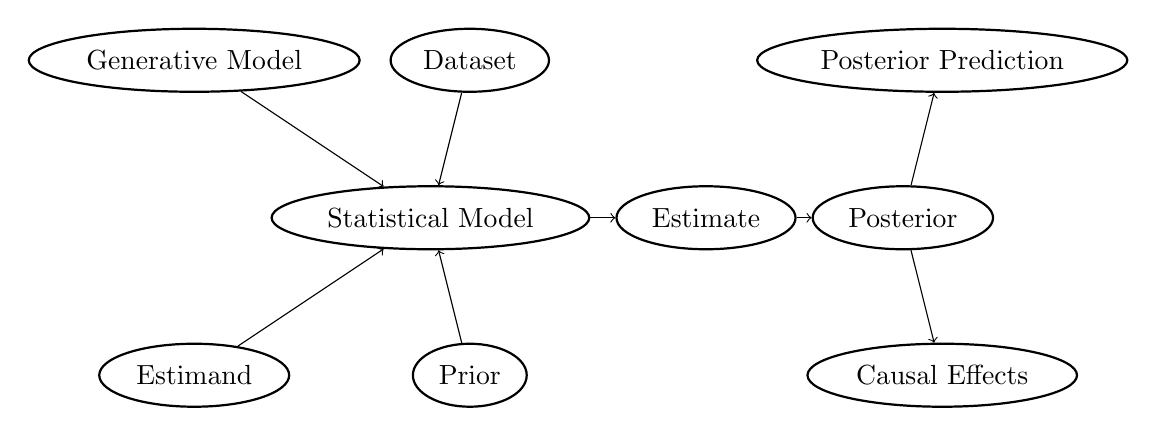
\begin{tikzpicture}[
    node distance=2cm,
    solid_node/.style={ellipse, draw, minimum size=8mm, thick},
    dashed_node/.style={ellipse, draw, dashed, minimum size=8mm, thick},
    directed/.style={-Stealth[scale=2], thick} 
]
        \node[solid_node] (G) at (0,4) {Generative Model};
        \node[solid_node] (Ed) at (0,0) {Estimand};
        \node[solid_node] (S) at (3,2) {Statistical Model};
        \node[solid_node] (Pi) at (3.5,0) {Prior};
        \node[solid_node] (D) at (3.5,4) {Dataset};
        \node[solid_node] (Et) at (6.5,2) {Estimate};
        \node[solid_node] (Po) at (9,2) {Posterior};
        \node[solid_node] (Pp) at (9.5,4) {Posterior Prediction};
        \node[solid_node] (CE) at (9.5,0) {Causal Effects};
    \draw [->] (G) -- (S);
    \draw [->] (Ed) -- (S);
    \draw [->] (Pi) -- (S);
    \draw [->] (D) -- (S);
    \draw [->] (S) -- (Et);
    \draw [->] (Et) -- (Po);
    \draw [->] (Po) -- (Pp);
    \draw [->] (Po) -- (CE);

    \end{tikzpicture}
    \caption{Core Bayesian Workflow, proposed in 305}
\end{figure}


The parameters in the dataset forms causal relationship in Fig. 2, based on my assumption. 
Publication and publication year can bias the proportion of Kozu obsidians. Although S, O and K can be related each other, I included single causality to be simple. 


\begin{figure}[H]
\centering 
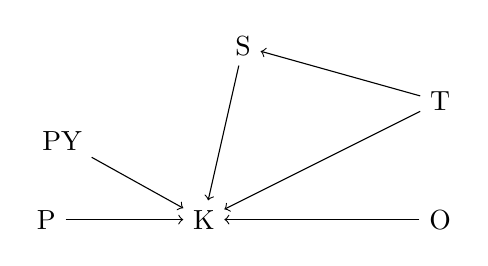
\begin{tikzpicture}[
    node distance=2cm,
    solid_node/.style={circle, draw, minimum size=8mm, thick},
    dashed_node/.style={circle, draw, dashed, minimum size=8mm, thick},
    directed/.style={-Stealth, thick} 
]
    \node (T) at (6,2.5) {T};
    \node (K) at (3,1) {K};
    \node (S) at (3.5,3.2) {S};
    \node (O) at (6,1) {O};
    \node (P) at (1,1) {P};
    \node (PY) at (1.2,2) {PY};
    \draw [->] (T) -- (S);
    \draw [->] (T) -- (K);
    \draw [->] (PY) -- (K);
    \draw [->] (S) -- (K);
    \draw [->] (P) -- (K);
    \draw [->] (O) -- (K);
\end{tikzpicture}
\caption{DAG of causalities among attributes of dataset - K: a ratio of Kouzu obsidians, S: a ratio of Shinshu obsidians, O: other sites, T: typology of artifacts or associated artifacts in the same layer, P: publication, PY: publication year.  }
\end{figure}
\newpage

Now, hypothesis of the analysis is sea level and proportion of Shinshu obsidians affect the Kozu obsidians to check the degree of influence. 
The parameters are T, K, S, dK, and dS. Y, SL, and U are hidden and do not exist in the data. U is the standard deviation of the model. 



\begin{figure}[H]
\centering 
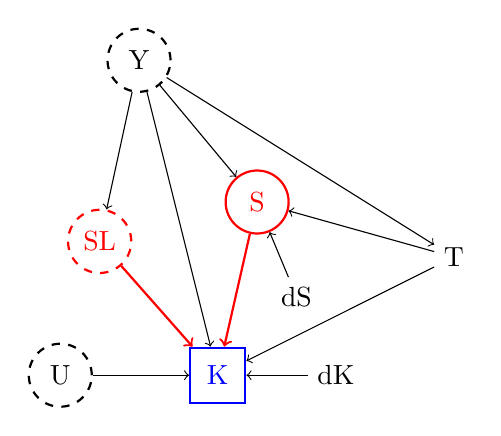
\begin{tikzpicture}[
    node distance=2cm,
    solid_node/.style={circle, draw, minimum size=8mm, thick},
    dashed_node/.style={circle, draw, dashed, minimum size=8mm, thick},
    directed/.style={-Stealth, thick} 
]
    \node[dashed_node] (Y) at (2,5) {Y};
    \node (T) at (6,2.5) {T};
    \node[dashed_node] (U) at (1,1) {U};
    \node[red, dashed_node] (SL) at (1.5,2.7) {SL};
    \node[blue, rectangle, draw, minimum size=7mm, thick] (K) at (3,1) {K};
    \node[red, solid_node] (S) at (3.5,3.2) {S};
    \node (dK) at (4.5,1) {dK};
    \node (dS) at (4,2) {dS};
    \draw [->] (Y) -- (T);
    \draw [->] (Y) -- (K);
    \draw [->] (Y) -- (S);
    \draw [->] (Y) -- (SL);
    \draw [->] (T) -- (S);
    \draw [->] (T) -- (K);
    \draw [->, red, thick] (SL) -- (K);
    \draw [->] (dS) -- (S);
    \draw [->] (dK) -- (K);
    \draw [->, red, thick] (S) -- (K);
    \draw [->] (U) -- (K);
\end{tikzpicture}
\caption{DAG of causalities among parameters - K: a ratio of Kouzu obsidians (blue solid square), S: a ratio of Shinshu obsidians (red dashed circle), SL: sea level difference based on current level (m; red dashed circle), T: typology of artifacts or associated artifacts in the same layer, dK: distance from Kozusima (km), dS: distance from the centre of Shinshu production sites (km), Y: true date (dashed circle as it is hidden), U: other hidden parameters influencing K (dashed). Colored arrows are from predictors to estimate. }
\end{figure}

\section{Three Models Proposed here}
As a background knowledge, we know the association of SL and Y based on previous research (). Therefore, multi-level modeling is used. 
The basic idea is that as T is observed parameter of Y, Y can be the True value of T, in other words. Then, I can make multilevel models, including Y predicts T to simulate the true Y values. As Y is estimated in ulam model of rethinking package, we can use it to estimate K, S, and SL.
The relationship between Y and T can be based on the Bayesian Analysis of Typological dates by Kanezaki, Omori, and Kobayashi in 2025 (\url{https://www.cambridge.org/core/journals/radiocarbon/article/optimal-bayesian-chronological-modeling-for-high-resolution-chronology-for-the-middle-jomon-of-kanto-region-honshu-island-japan-approaching-a-generational-scale/4B1717D6D82FFA1CF8A63E6B1EBCCC8D}). 
However, in this case, T is modeled simple poisson distribution with 25 phases.


\begin{figure}[H]
\centering 
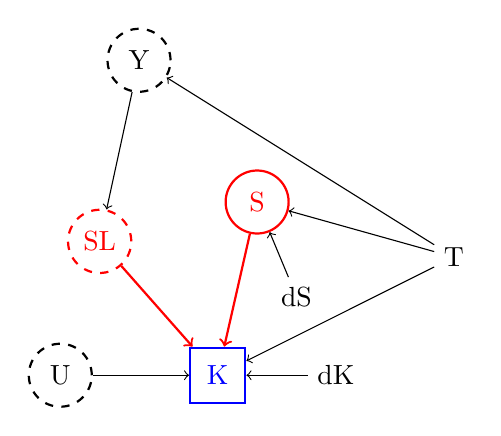
\begin{tikzpicture}[
    node distance=2cm,
    solid_node/.style={circle, draw, minimum size=8mm, thick},
    dashed_node/.style={circle, draw, dashed, minimum size=8mm, thick},
    directed/.style={-Stealth, thick} 
]
    \node[dashed_node] (Y) at (2,5) {Y};
    \node (T) at (6,2.5) {T};
    \node[dashed_node] (U) at (1,1) {U};
    \node[red, dashed_node] (SL) at (1.5,2.7) {SL};
    \node[blue, rectangle, draw, minimum size=7mm, thick] (K) at (3,1) {K};
    \node[red, solid_node] (S) at (3.5,3.2) {S};
    \node (dK) at (4.5,1) {dK};
    \node (dS) at (4,2) {dS};
    \draw [->] (T) -- (Y);
    \draw [->] (Y) -- (SL);
    \draw [->] (T) -- (S);
    \draw [->] (T) -- (K);
    \draw [->, red, thick] (SL) -- (K);
    \draw [->] (dS) -- (S);
    \draw [->] (dK) -- (K);
    \draw [->, red, thick] (S) -- (K);
    \draw [->] (U) -- (K);
\end{tikzpicture}
\caption{DAG of causalities among parameters - K: a ratio of Kouzu obsidians (blue solid square), S: a ratio of Shinshu obsidians (red dashed circle), SL: sea level difference based on current level (m; red dashed circle), T: typology of artifacts or associated artifacts in the same layer, dK: distance from Kozusima (km), dS: distance from the centre of Shinshu production sites (km), Y: true date (dashed circle as it is hidden), U: other hidden parameters influencing K (dashed). Colored arrows are from predictors to estimate. }
\end{figure}

\begin{itemize}
    \item Model 1: stratifies data by T, and includes all the causation in Fig. 3: Model T by Y, Model SL by Y, Model S by Y and dS, Model K by S, SL, Y, dK, and U. 

    \item Model 2: stratifies data by T, and includes all the causation in Fig. 4: Model T by Y, Model SL by Y, Model S by dS, Model K by S, SL, Y, dK, and U with correlation between S and SL.
    \begin{itemize}
        \item Although Model 2 does not rely on Y to predict S, the causation is represented as correlation between S and SL. 
    \end{itemize} 
    \item Model 3: includes all the causation in Fig. 3 without any stratification: Model T by Y, Model SL by Y, Model S by Y and dS, Model K by S, SL, Y, dK, and U. 
    \begin{itemize}
        \item See the m.Rmd and m.html
    \end{itemize}
\end{itemize}

\newpage

\section{The priors and statistical model for Model 1 (m1)}
- This model stratifies S, SL, and Y and includes hierarchical models of S and SL by Y
\begin{itemize}
\item Model K
$$K \sim Normal(\mu_K, U) $$
$$logit(\mu_K) = \alpha _{K}[T] + \beta _{K_S}[T] \cdot S + \beta _{K_{SL}}[T] \cdot SL + \beta _{K_{dK}} * dK$$

\begin{itemize}
    \item We do not know anything about this but think similar for all group. 
    \item So use partial pooling to regularize the estimate. 
    \item mean should start at 0 and has small variation.
    \item In this case (m1), we do not include correlation. 
    \item This is because multilevel models of S and SL includes the information of Y 
    \item But we have to regularize.
\end{itemize}
$$\alpha _K = \overline{\alpha _K} + \sigma_{\alpha _K} * z_{\alpha _K}[T] $$
$$\beta _{K_S } = \overline{\beta _{K _S}} + \sigma_{\beta _{K _S}} * z_{\beta _{K_S}}[T] $$
$$\beta _{K_SL } = \overline{\beta _{K _{SL}}} + \sigma_{\beta _{K _{SL}}} * z_{\beta _{K_{SL}}}[T] $$
$$\beta _{K_Y } = \overline{\beta _{K _Y}} + \sigma_{\beta _{K _Y}} * z_{\beta _{K_Y}}[T] $$

$$\overline{\alpha _K}, \overline{\beta _{K _S}}, \overline{\beta _{K _{SL}}}, \overline{\beta _{K _Y}} \sim Normal(0,0.3)$$
$$\sigma_{\alpha _K}, \sigma_{\beta _{K _S}}, \sigma_{\beta _{K _{Sl}}}, \sigma_{\beta _{K _Y}} \sim Exponential(1)$$
$$z_{\alpha _K}[T] \sim Normal(0,0.1)$$
$$z_{\beta _{K_S}}[T]  \sim Normal(0,0.1)$$
$$z_{\beta _{K_{SL}}}[T]  \sim Normal(0,0.1)$$
$$z_{\beta _{K_Y}}[T]  \sim Normal(0,0.1)$$


$$\beta _{K_S}, \beta _{K_SL} \sim MultiNormal(\overline{\beta _b{K_S}}, \overline{\beta _b{K_SL}}, \rho _{S, SL}, \sigma _{S, SL})$$
$$\overline {\beta _{K_S}}, \overline{\beta _{K_SL}} \sim Normal(0, 0.3)$$
$$ \rho _{S, SL} \sim lkj_corr(1) $$
$$\sigma _{S, SL} \sim Exponential(2) $$
\begin{itemize}
    \item Followings don't need regularization
    \item We are hoping/believing $b_{dK}$ is negative, but this is not prior. 
\end{itemize}
$$\beta _{K_{dK}} \sim Normal(0, 0.5)$$
$$U \sim Exponential(1)$$


\item Model S 
$$S \sim Normal(\mu_S, \sigma_S)$$
$$logit(\mu_S) = \alpha _S [T] + \beta _ {S_{dS}} * dS$$
\begin{itemize}
    \item I am hoping/believing $\beta_{dS}$ is negative and $\beta_{Y_S}$ is positive 
    \item partial pooling for the same reason for $\alpha_S$ and $\beta _{Y_S}$
\end{itemize}
$$\alpha_S = \overline{\alpha _S} + \sigma_{\alpha _S} * z_{\alpha _S}[T]$$
$$\beta _{S_Y} = \overline{\beta _{S_Y}} + \sigma _{\beta _{S_Y}} * z _ {\beta _{S_Y}}[T]$$

$$\overline{\alpha _S}, \overline{\beta _{S_Y}} \sim Normal(0,0.1)$$
$$\sigma_{\alpha _S}, \sigma _{\beta _{S_Y}} \sim Exponential(6)$$
$$z_{\alpha _S}[T] \sim Normal(0,0.05)$$
$$z _{\beta _{S_Y}}[T] ~ normal(0,0.05)$$

\begin{itemize}
    \item don't need regularization
\end{itemize}
$$\beta {S_{dS}} \sim Normal(0,0.1)$$
$$\sigma_S \sim Exponential(1)$$


\item Model SL by Y 
\begin{itemize}
    \item The log function and prior was refered to the previous research of Sea Level Change over time. 
    \item This function is abstruct so I will have to actually stan code to provide accurate estimates
    \item ulam code in r does not allow us to hartd code the conditional function. 
    \item vector[200]: SL ~ normal(muSL + aSL2, sigmaSL),
\end{itemize}
$$SL \sim Normal(\mu_{SL}, \sigma_{SL})$$
$$logit(\mu_{SL}) = \alpha _{SL} + Y[i] * \beta_ {SL}$$
$$\alpha _{SL} \sim Normal(8, 0.01)$$
$$\beta _{SL} \sim Normal(0.8, 0.01)$$
$$\sigma_{SL} \sim Exponential(1)$$

\item Model T by Y  
$$T \sim Poisson((Y + 16)/ ( -2.4 + 16) * 25)$$
\begin{itemize}
    \item This should be hard coded based on the previous research (Kanezaki, et al., 2025)
\end{itemize}

\item Model Y randomly
$$Y \sim Uniform( -16 , -2.4 )$$
\end{itemize}


\newpage

\section{The priors and statistical model for Model 2 (m2)}
- This model stratifies S, SL, and Y and includes correlation between S and SL. 

\begin{itemize}
 \item Main model K

$$K \sim Normal(\mu_K, U) $$
$$logit(\mu_K) = \alpha _{K}[T] + \beta _{K_S}[T] \cdot S + \beta _{K_{SL}}[T] \cdot SL + \beta _{K_{dK}} * dK$$
\begin{itemize}
    \item We do not know anything about this but think similar for all group. 
    \item So use partial pooling to regularize the estimate. 
    \item mean should start at 0 and has small variation.
    \item In this case (m2), we do include correlation between S and SL due to Y. 
\end{itemize}
$$\alpha _K = \overline{\alpha _K} + \sigma_{\alpha _K} * z_{\alpha _K}[T] $$
$$\overline{\alpha _K} \sim Normal(0,0.3)$$
$$\sigma_{\alpha _K} \sim Exponential(1)$$
$$z_{\alpha _K}[T] \sim Normal(0,0.1)$$
\begin{itemize}
    \item correlaton between $\beta _{K_S}$ and $\beta _{K_SL}$
    \item this is not too strong but good correlation
\end{itemize}
$$\beta _{K_S}, \beta _{K_SL} \sim MultiNormal(\overline{\beta _b{K_S}}, \overline{\beta _b{K_SL}}, \rho _{S, SL}, \sigma _{S, SL})$$
$$\overline {\beta _{K_S}}, \overline{\beta _{K_SL}} \sim Normal(0, 0.3)$$
$$ \rho _{S, SL} \sim lkj_corr(1) $$
$$\sigma _{S, SL} \sim Exponential(2) $$
\begin{itemize}
    \item Followings don't need regularization
    \item We are hoping/believing $b_{dK}$ is negative, but this is not prior. 
\end{itemize}
$$\beta _{K_{dK}} \sim Normal(0, 0.5)$$
$$U \sim Exponential(1)$$


\item Model S 
$$S \sim Normal(\mu_S, \sigma_S)$$
$$logit(\mu_S) = \alpha _S [T] + \beta _ {S_{dS}} * dS$$
\begin{itemize}
    \item I am hoping/believing $\beta_{dS}$ is negative and $\beta_{Y_S}$ is positive 
    \item partial pooling for the same reason for $\alpha_S$ and $\beta _{Y_S}$
\end{itemize}
$$\alpha_S = \overline{\alpha _S} + \sigma_{\alpha _S} * z_{\alpha _S}[T]$$
$$\beta _{S_Y} = \overline{\beta _{S_Y}} + \sigma _{\beta _{S_Y}} * z _ {\beta _{S_Y}}[T]$$

$$\overline{\alpha _S}, \overline{\beta _{S_Y}} \sim Normal(0,0.1)$$
$$\sigma_{\alpha _S}, \sigma _{\beta _{S_Y}} \sim Exponential(6)$$
$$z_{\alpha _S}[T] \sim Normal(0,0.05)$$
$$z _{\beta _{S_Y}}[T] ~ normal(0,0.05)$$

\begin{itemize}
    \item don't need regularization
\end{itemize}
$$\beta {S_{dS}} \sim Normal(0,0.1)$$
$$\sigma_S \sim Exponential(1)$$


\item Model SL by Y 
\begin{itemize}
    \item The log function and prior was refered to the previous research of Sea Level Change over time. 
    \item This function is abstruct so I will have to actually stan code to provide accurate estimates
    \item ulam code in r does not allow us to hartd code the conditional function. 
    \item vector[200]: SL ~ normal(muSL + aSL2, sigmaSL),
\end{itemize}
$$SL \sim Normal(\mu_{SL}, \sigma_{SL})$$
$$logit(\mu_{SL}) = \alpha _{SL} + Y[i] * \beta_ {SL}$$
$$\alpha _{SL} \sim Normal(8, 0.01)$$
$$\beta _{SL} \sim Normal(0.8, 0.01)$$
$$\sigma_{SL} \sim Exponential(1)$$

\item Model T by Y  
$$T \sim Poisson((Y + 16)/ ( -2.4 + 16) * 25)$$

\item Model Y randomly
$$Y \sim Uniform( -16 , -2.4 )$$

\end{itemize}

\newpage

\section{The priors and statistical model for Model 1 (m1)}

\begin{itemize}
\item Model K
$$K \sim Normal(\mu_K, U) $$
$$logit(\mu_K) = \alpha _{K}[T] + \beta _{K_S}[T] \cdot S + \beta _{K_{SL}}[T] \cdot SL + \beta _{K_{dK}} * dK +  \beta _{K_T}[T]$$
\begin{itemize}
    \item We do not know anything about this but think similar for all group. 
    \item So use partial pooling to regularize the estimate. 
    \item mean should start at 0 and has small variation.
\end{itemize}

$$\alpha _K, \beta _{K_S }, \beta _{K_SL }, \beta _{K_Y }, \beta _{K_{dK}}  \sim Normal(0,0.3)$$


$$\beta _{K_T} = \overline{\beta _{K_T}} + \sigma_{\beta _{K_T}} * z_{\beta_{K_T}}[T]$$
\begin{itemize}
    \item regularization
\end{itemize}
$$\overline{\beta {K_T}} \sim Normal(0, 0.3)$$
$$\sigma_{\beta _{K_T}} \sim Exponential(6)$$
$$z_{\beta _{K_T}}[T] \sim Normal(0, 1)$$

$$U \sim Exponential(1)$$


\item Model S 
$$S \sim Normal(\mu_S, \sigma_S)$$
$$logit(\mu_S) = \alpha _S [T] + \beta _ {S_{dS}} * dS + \beta_{S_T}$$
\begin{itemize}
    \item I am hoping/believing $\beta_{dS}$ is negative and $\beta_{Y_S}$ is positive 
    \item partial pooling for the same reason for $\alpha_S$ and $\beta _{Y_S}$
\end{itemize}
$$\alpha_S, \beta _{S_Y}, \beta {S_{dS}} \sim Normal(0,0.1)$$

$$\beta _{S_T} = \overline{\beta _{S_T}} + \sigma_{\beta _[S_T]} * z_{\beta{S_T}}[T]$$
$$\overline{\beta _{S_T}} \sim Normal(0, 0.001)$$
$$\sigma_{\beta _[S_T]} \sim Exponential(10)$$ 
$$z_{\beta{S_T}}[T] \sim Normal(0, 0.1)$$

$$\sigma_S \sim Exponential(1)$$


\item Model SL by Y 
\begin{itemize}
    \item The log function and prior was refered to the previous research of Sea Level Change over time. 
    \item This function is abstruct so I will have to actually stan code to provide accurate estimates
    \item ulam code in r does not allow us to hartd code the conditional function. 
    \item vector[200]: SL ~ normal(muSL + aSL2, sigmaSL),
\end{itemize}
$$SL \sim Normal(\mu_{SL}, \sigma_{SL})$$
$$logit(\mu_{SL}) = \alpha _{SL} + Y[i] * \beta_ {SL}$$
$$\alpha _{SL} \sim Normal(8, 0.01)$$
$$\beta _{SL} \sim Normal(0.8, 0.01)$$
$$\sigma_{SL} \sim Exponential(1)$$

\item Model T by Y  
$$T \sim Poisson((Y + 16)/ ( -2.4 + 16) * 25)$$
\begin{itemize}
    \item This should be hard coded based on the previous research (Kanezaki, et al., 2025)
\end{itemize}

\item Model Y randomly
$$Y \sim Uniform( -16 , -2.4 )$$

\end{itemize}




\end{document}
